\chapter{Toteutus}
\label{ch:toteutus}
Tässä osiossa käydään läpi kappaleessa \ref{ch:suunnittelu} suunniteltun ohjelman toteuttaminen. Esitys alkaa yleiskuvalla toteutuksen komponenteista ja niiden toiminnasta. Yleiskuvan jälkeen mennään tarkemmin ohjelman yksityiskohtiin kuten kirjastoihin ja niiden toimintaan. Lopuksi mietitään jatkokehitysideoita, mitä olisi voinut lisätä, tehdä toisin ja mahdollisia puutteita.


\section{Yleiskuva}
\label{ch:rcb-sub-yleiskuva}
Ohjelman tarkoitus oli tilata IED-laitteen viestit ja prosessoida ne JSON-muotoon RabbitMQ-palvelimelle. RabbitMQ:lta muut ohjelmat pystyivät tilaamaan JSON-viestejä. Kuvassa \ref{fig:rcb-sub-komponenttikaavio} on esitetty komponenttikaavio  toteutetusta ohjelmasta ja siihen käytetyistä kirjastoista. Toteutettu komponentti on kuvassa keskellä keltaisella ja nimeltään \emph{rcb\_sub}. Kuvasta voi nähdä miten eri komponentit ovat relaatiossa keskenään rcb\_sub-ohjelman kanssa. Kuvassa on myös esitetty IED-laite ja RabbitMQ-palvelin. Rcb\_sub toteutettiin Linux-käyttöjärjestelmälle komentoriviohjelmana ilman käyttöliittymää.

\begin{figure}[ht!]
	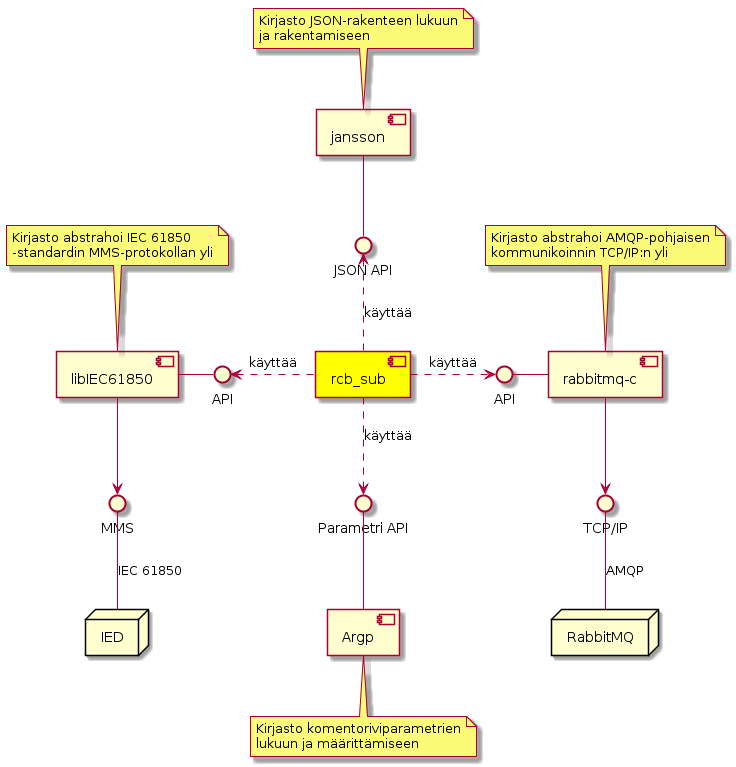
\includegraphics[width=1\textwidth]{pictures/rcb-sub-component-diagram.png}
	\caption{Toteutuksen komponenttikaavio sen osista ja relaatioista toisiinsa.}
	\label{fig:rcb-sub-komponenttikaavio}
\end{figure}

Toteutuksessa käytettiin seuraavia kirjastoja:
\begin{itemize}
	\item \emph{libIEC61850},
	\item \emph{rabbitmq-c},
	\item \emph{jansson}, ja
	\item \emph{Argp}.
\end{itemize}
Kaikki käytetyt kirjastot on toteutettu C-kielellä, kuten rcb\_sub. Kirjastojen tarkoitus on abstrahoida jonkin asian käyttö, ja tarjota käyttäjälle siitä helppokäyttöinen ja ymmärrettävä rajapinta. Rajapintaa käyttämällä kirjasto hoitaa matalan tason toiminnan ilman, että sen käyttäjän tarvitsee siitä välittää. LibIEC61850-kirjasto abstrahoi IEC 61850 -standardin käyttöä ja hoitaa matalan tason MMS-protokollan kommunikoinnin \mbox{\cite{libIEC61850-repo}}. Samaa kirjastoa käytettiin demoversiossa (kappale \ref{ch:demoversio-ja-sen-toiminta}) ja kirjaston kerrosarkkitehtuuri esitettiin aikaisemmin kuvassa \ref{fig:libiec61850-layer-architecture}. Kuvassa \ref{fig:rcb-sub-komponenttikaavio} libIEC61850 kommunikoi suoraan IED\--\-lait\-teen kanssa MMS-protokollaa käyttäen. Rabbitmq-c-kirjasto abstrahoi RabbitMQ-palvelimen käyttöä ja hoitaa matalan tason AMQP-pohjaisen kommunikoinnin \mbox{\cite{rabbitmq-c-repo}}. Toteutuksessa rabbitmq-c kommunikoi suoraan RabbitMQ-palvelimen kanssa. Jansson-kirjasto abstrahoi JSON-rakenteiden lukua ja käsittelyä C-kielelle \mbox{\cite{jansson-repo}}. Kirjastoa käytettiin rakentamaan IED-\-lait\-teel\-ta saapuneesta viestistä JSON-muotoinen viesti. JSON-rakenne on nähtävissä liitteessä \ref{ch:report-json-format}. Argp-kirjasto auttaa ohjelman komentoriviparametrien määrittämisessä ja käsittelyssä \mbox{\cite{argp-glibc-guide}}. Kirjastolla voidaan toteuttaa \emph{UNIX}-tyyliset \emph{parametrit} (engl. \emph{arguments}) ja \emph{valitsimet/vivut} (engl. \emph{options/switches}). Esimerkki parametreistä on Linux-komento \texttt{mv foo.txt bar.txt}, jossa \emph{foo.txt} ja \emph{bar.txt} ovat parametreja mv-ohjelmalle. Vivut voidaan ohjelmalle antaa lyhyessä tai pitkässä muodossa. Esimerkkinä lyhyistä ja pitkistä vivuista \texttt{-b} ja \texttt{-{}-bytes} vastaavasti. Vivut voivat myös vaatia parametreja toimiakseen. Parametri voidaan kirjoittaa lyhyen vivun perään välilyönnilla tai ilman. Pitkän vivun kanssa se erotetaan välilyönillä tai yhtäsuuruusmerkillä (=). Esimerkkinä lyhyestä \texttt{-w 5} ja pitkästä \texttt{--width=5}, jossa width-vivulle annetaan parametrina 5. Kirjasto lisää ohjelmaan automaattisesti Linuxista käyttäjille tutut \texttt{-{}-help} ja \texttt{-{}-version} vivut. Vivulla \texttt{-{}-help} kirjasto tulostaa Linuxilta tutun ohjelman aputekstin käyttäjälle, jossa on esitetty sen kaikki parametrit, vivut ja niiden selitteet \mbox{\cite{step-by-step-into-argp}}.

Kuvassa \ref{fig:rcb-sub-sekvenssikaavio} on esitetty rcb\_sub-ohjelman sekvenssikaavio pääpiirteisestä toiminnasta. Toteutus noudattaa suurinpiirtein samoja periaatteita kuin demo (kuva \ref{fig:sequence-diagram-report-subscription}). Tässä kohtaa käydään läpi ohjelman pääpiirteinen toiminta ja myöhemmin tarkemmin läpi kappaleessa \ref{rcb-sub-toiminta}. Ensin ohjelman suoritus alkaa lukemalla annetut parametrit ja vivut Argp-kirjastolla (kohdat 1--2). Parametreissa tulee tiedot yhteyden muodostamiseen IED-laitteelle ja RabbitMQ-palvelimelle (kohdat 3--6). Parametreissa on myös tiedot RCB-instansseista jotka halutaan IED:ltä tilata. RCB-instanssien määrä voi vaidella IED-laitteiden välillä. Tämän työn tapauksessa määrät vaihtelivat vällillä 3--13. Yhteyksien muodostamisen jälkeen jokainen parametrina annettu RCB käydään läpi silmukassa ja sen arvot ja datajoukon viitteet luetaan IED:ltä (kohdat 7--12). Tämän jälkeen sisäkkäisessä silmukassa luetaan datajoukon viitteiden muuttujien \emph{spesifikaatiot} (kohdat 11--12). Spesifikaatio antaa tiedot muuttujien pituudesta ja tyypistä. Näitä tietoja käytettiin JSON-rakenteessa täydentämään viestiä (esimerkkinä liiteessä \ref{ch:report-json-format} rivit 21--22). Tämän jälkeen tehdään toinen silmukka, jossa jokainen RCB-instanssi tilataan ja niille asetetaan takaisinkutsufunktio (kohdat 13--16). Arvojen kirjoitushetkellä (kohta 15) RCB varataan ja se aloittaa viestien lähettämisen rcb\_sub-ohjelmalle. Jokaisen RCB:n kirjoituksen jälkeen ohjelma jää loputtomaan silmukkaan ottamaan viestejä vastaan (kohdat 17--22). Viestin saapuessa kutsutaan asetettua takaisinkutsufunktiota, jonka parametrina on saapunut viesti (kohta 17). Viesti muutetaan JSON-muotoon jansson-kirjastolla ja julkaistaan RabbitMQ-palvelimelle rabbitmq-c-kirjastolla (kohdat 18--21).

\begin{figure}[ht!]
	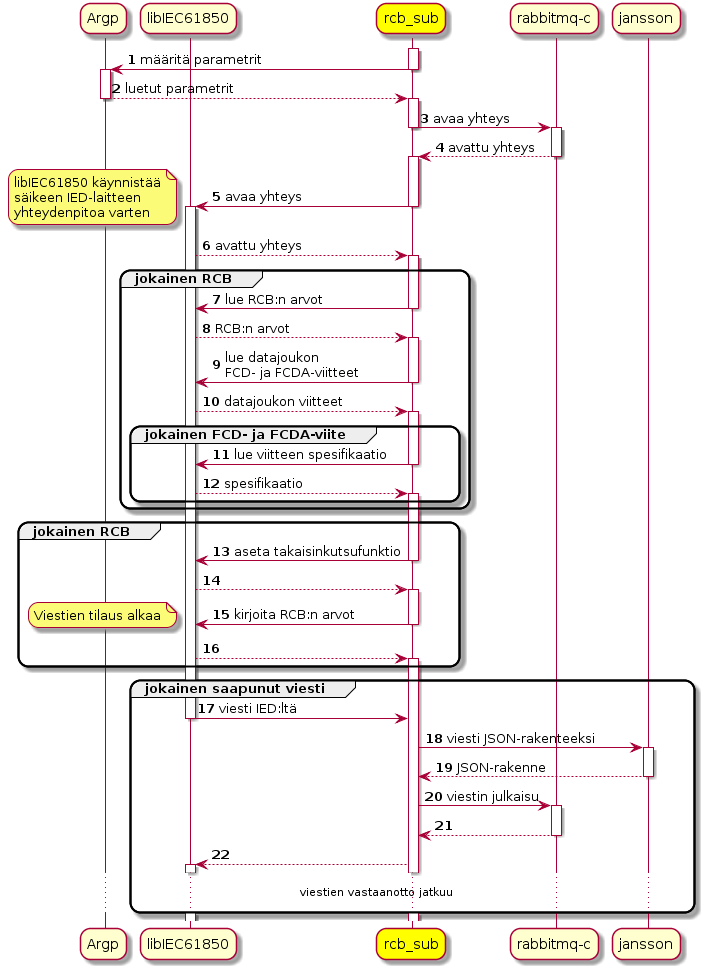
\includegraphics[width=1\textwidth]{pictures/rcb-sub-general-sd.png}
	\caption{Sekvenssikaavio rcb\_sub-ohjelman kokonaistoiminnasta.}
	\label{fig:rcb-sub-sekvenssikaavio}
\end{figure}


\section{Ohjelman toiminta}
\label{rcb-sub-toiminta}
Tulevissa kappaleissa käydään läpi yksityiskohtaisemmin rcb\_sub-ohjelman toimintaa, joka esiteltiin pääpiirteittäin kappaleessa \ref{ch:rcb-sub-yleiskuva}. Kappaleiden järjestys noudattaa kuvassa \ref{fig:rcb-sub-sekvenssikaavio} olevan sekvenssikaavion järjestystä. Toisin sanoen ohjelmaa käydään tarkemmin läpi sen suorituksen järjestyksessä.


\subsection{Parametrisointi}
Ohjelma parametrisoitiin Argp-kirjastolla. Kirjasto tarjoaa rajapinnan komentoriviparametrien käsittelyyn ja määrittämiseen. Parametrien muodot ovat tutut muista Linux-käyt\-tö\-jär\-jes\-tel\-män parametreista ja samaa periaatetta käytettiin tässäkin ohjelmassa. Kirjasto myös lisäsi ohjelmaan automaattisesti aputekstin käyttäjää varten. Aputeksti sisältää tietoa ohjelman parametreista ja niiden käytöstä. Aputekstin pystyi tulostamaan vivulla \texttt{-{}-help}. Liitteessä \ref{ch:rcb-sub-help-output} on esitetty miltä ohjelman aputeksti näyttää. Liitteestä voi myös nähdä kaikki ohjelman parametrit ja lyhyen selityksen mihin kutakin käytetään.

Ohjelmiston parametrien ja vipujen voidaan ajatella koostuvan kolmesta eri ryhmästä (katso liite \ref{ch:rcb-sub-help-output} rivit 1--4). Ensin päätason vaihtoehtoiset vivut \texttt{OPTIONS} (rivi 1). Pakolliset parametrit \texttt{EXCHANGE} ja \texttt{ROUTING\_KEY} (rivi 2). Viimeisenä ryhmänä \texttt{RCB\_REF} parametri ja siihen liittyvät vivut \texttt{RCB\_OPTIONS} (rivi 3). Näitä ryhmiä voi olla n-kappaletta, mutta vähintään yksi. Liitteessä \ref{ch:rcb-sub-help-output} riveillä 71--72 on esitetty esimerkki, joka tilaa viestit IED-laitteelta osoitteesta 192.168.2.220. AMQP-vaihteen nimi on \emph{testexchange} ja reititysavaimen nimi on \emph{testkey}. IED-laitteelta tilataan RCB-instanssi viitteellä MY\_LD0\-/\-LLN0\-.\-BR\-.\-rcbMeas01. Instanssille asetetaan yleinen kysely (\texttt{-g1}), liipaisimet (\texttt{-t27}) ja viestin vaihtoehtoiset kentät (\texttt{-o16}). Liipaisimet ja vaihtoehtoiset kentät annetaan numeroarvoilla summaamalla niitä yhteen. Vaihtoehdot näkee ohjelman aputekstistä (esimerkiksi liipaisimet riveillä 53--58).

Suurin osa \texttt{OPTION} vivuista ovat itsestäänselviä. Esimerkkinä \texttt{-{}-amqp-host}, joka kertoo A\-M\-Q\-P-pal\-ve\-li\-men IP-osoitteen, ja \texttt{-{}-ied-host}, joka kertoo IED-laitteen IP-osoitteen. Parametrit \texttt{EXCHANGE} ja \texttt{ROUTING\_KEY} määrittävät nimet RabbitMQ-palvelimen vaihteelle ja reititysavaimelle. Parametri \texttt{RCB\_REF} määrittää viitteen tilattavaan RCB-instanssiin IED-laitteella. Tätä seuraa vaihtoehtoinen \texttt{RCB\_OPTIONS} vipu, joka määrittää edeltävän instanssin kirjoitettavat arvot ennen tilausta. Sillä voidaan määrittää käytetyt vaihtoehtoiset kentät (\texttt{-{}-opt-fields}), käytetyt liipaisimet (\texttt{-{}-trigger}) ja pyydetäänkö yleistä kyselyä ennen muita viestejä (\texttt{-{}-gi}). Liipaisimien nimet vastaavat aikaisemmin kappaleessa \ref{ch:rcb-toiminta} esitettyjä arvoja ja numeeriset arvot tulevat libIEC61850-kirjastosta. Vaihtoehtoisten kenttien nimet vastaavat aikaisemmin taulukossa \ref{tab:iec61850-optional-fields-definition} esitettyjä arvoja ja numeeriset arvot tulevat myös libIEC61850-kirjastosta.

\subsection{Yhteyksien muodostus}
Parametrien luvun jälkeen ohjelma muodostaa yhteydet ensin RabbitMQ-palvelimelle ja sen jälkeen IED-laitteelle. Kuvassa \ref{fig:rcb-sub-open-connections} on esitetty sekvenssikaavio, joka näyttä mitä kirjaston funktioita ohjelma kutsuu missäkin järjestyksessä. Funktiot ja niiden parametrit voi tarkemmin tarkistaa kirjaston omasta dokumentaatiosta. Tämä tarkentaa yleiskuvasta \ref{fig:rcb-sub-sekvenssikaavio} kohdat 3--6. Kaaviossa ohjelma muodostaa yhteydet vain kerran. Ohjelma on kuitenkin toteutettu niin, että se yrittää muodostaa yhteydet uudestaan vikatilanteissa. Jos muodostus ei onnistu, ohjelma kirjoittaa lokin tapahtuneesta ja odottaa hetken ennen uudelleen yritystä.

\begin{figure}[ht!]
	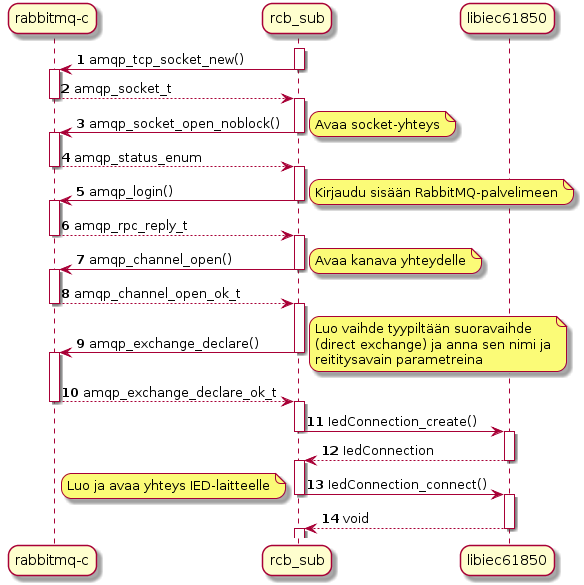
\includegraphics[width=1\textwidth]{pictures/rcb-sub-open-connections.png}
	\caption{Sekvenssikaavio kuinka rcb\_sub avaa yhteydet RabbitMQ-palvelimelle ja IED-laitteelle.}
	\label{fig:rcb-sub-open-connections}
\end{figure}

Yhteyden avauksen ja sisäänkirjautumisen jälkeen ohjelma avaa kanavan kohdassa 7--8. Kanava on yhteyden päälle avattu oma erillinen kommunikointiväylä, joka ei sotkeudu muihin kanaviin. Yhteen avattuun yhteyteen voi olla avattuna monta eri kanavaa. Kanavat mahdollistavat monen eri säikeen jakaa sama yhteys, ilman että tieto voi vuotaa toiseen säikeeseen. Kohdassa 9 kutsutaan funktiota \texttt{amqp\_exchange\_declare()}. Funktio määrittää vaihteen tyyppiä suoravaihde RabbitMQ-palvelimelle. Suoravaihde käsiteltiin kappaleessa \ref{ch:direct-exchange}. Ohjelmaan ei toteutettu parametria vaihdetyypin määrittämiseen, koska katsottiin että suoravaihde on riittävä nykyisten vaatimusten täyttämiseksi. Tulevaisuudessa voidaan tarvittaessa lisätä parametrit vaihdetyypin vaihtamiseen.


\subsection{IED:n attribuuttien tyyppin ja koon luku}
Yhteyksien muodostamisen jälkeen ohjelma käy läpi silmukassa jokaisen parametrina annetun RCB:n viitteen. Lukee RCB:n datajoukon viitteet ja selvittää jokaisen viitatun attribuutin spesifikaatiot, eli sen oikean viitteen, tyypin ja koon. Kuvassa \ref{fig:rcb-sub-reading-specifications} on esitetty sekvenssikaavio kuinka rcb\_sub tämän tekee libIEC61850-kirjaston avulla. Kuva tarkentaa yleiskuvassa \ref{fig:rcb-sub-sekvenssikaavio} kohtia 7--12.

\begin{figure}[ht!]
	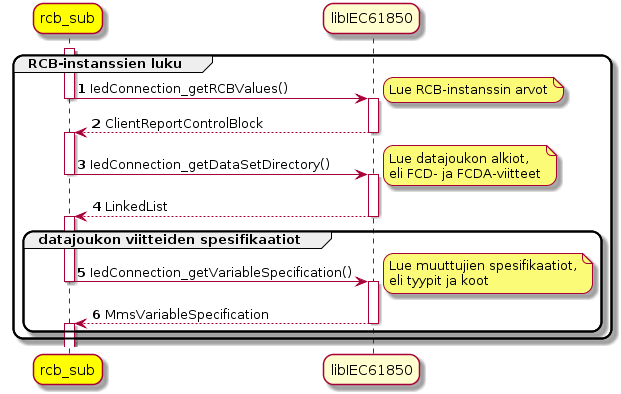
\includegraphics[width=1\textwidth]{pictures/rcb-sub-reading-specifications.png}
	\caption{Sekvenssikaavio kuinka rcb\_sub lukee RCB-instanssin arvot ja muuttujien spesifikaatiot.}
	\label{fig:rcb-sub-reading-specifications}
\end{figure}

Ensin RCB:sta luetaan sen tiedot IED-laitteelta (kohdat 1--2). RCB:ltä saadaan tieto mihin datajoukkoon se on liitetty. Tätä käsiteltiin kappaleessa \ref{ch:rcb-toiminta} ja taulukossa \ref{tab:iec61850-brcb-class-definition} kenttä \emph{DatSet}, joka kertoo käytetyn datajoukon viitteen. Tällä tiedolla ohjelma voi lukea datajoukon FCD- ja FCDA-viitteet (kohdat 3--4). Tästä saadaan jokainen viite listassa, joka käydään läpi silmukassa kohdissa 5--6. Jokaiselle viitteelle luetaan sen spesifikaatio. Spesifikaatiorakenne sisältää sisäkkäisiä spesifikaatioita, jos viite viittaa moneen muuttujaan IED-laitteen hierarkiassa. Tämä tapahtuu samalla periaatteella, jolla FCD- ja FCDA-viitteet viittaavaat moneen muuttujaan hierarkiassa alaspäin. Kuinka FCD- ja FCDA-viitteet toimivat käsiteltiin kappaleessa \ref{ch:fc-and-dataset}. Jokainen luettu viite tallennetaan ja niitä käytetään myöhemmin viestin kanssa JSON-rakenteessa. Esimerkkinä liitteessä \ref{ch:report-json-format} riveillä 21--22 tyyppi ja koko -tiedot.


\subsection{Viestien tilaus}
Ohjelman luettua kaikki muuttujien spesifikaatiot. Ohjelma tilaa silmukassa kaikki parametrina annetut RCB-instanssit. Kuvassa \ref{fig:rcb-sub-subscribe-reports} on esitetty sekvenssikaavio, kuinka rcb\_sub tilaa RCB-instanssit libIEC61850-kirjaston avulla. Kuva tarkentaa yleiskuvassa \ref{fig:rcb-sub-sekvenssikaavio} kohtia 13--16.

\begin{figure}[ht!]
	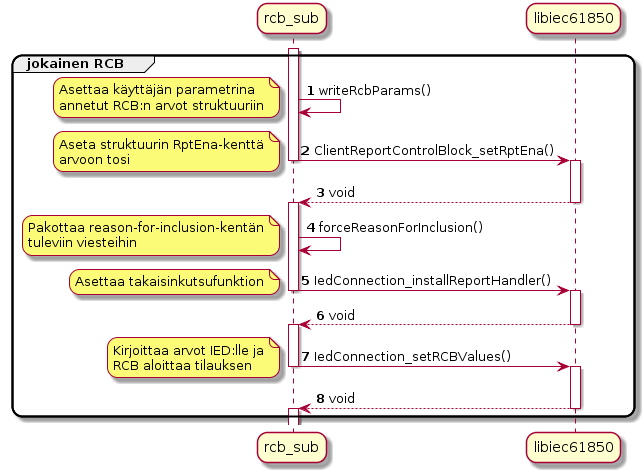
\includegraphics[width=1\textwidth]{pictures/rcb-sub-subscribe-reports.png}
	\caption{Sekvenssikaavio kuinka rcb\_sub tilaa RCB-instanssit.}
	\label{fig:rcb-sub-subscribe-reports}
\end{figure}

Ohjelma käsittelee libIEC61850-kirjaston tarjoamaa \emph{ClientReportControlBlock} struktuurin instanssia. Kirjasto palauttaa struktuurin instanssin, kun RCB:n arvot luetaan IED-laitteelta. Kaikki RCB:lle kirjoitettavat arvot asetetaan instanssiin ennen IED-laitteelle kirjoitusta. Näitä arvoja ovat ohjelmalle parametreinä annetut arvot, kuten liipaisimet ja vaihtoehtoiset kentät. Tämän ohjelma tekee kutsumalla omaa funktiota \texttt{wri\-teRcb\-Pa\-rams\-()} (kohta 1). Tämän jälkeen ohjelma asettaa RCB:n \emph{RptEna}-kentän arvoksi tosi (kohdat 2--3). Tämä kenttä kontrolloi RCB-instanssin varausta ja onko tilaus päällä. Seuraavaksi ohjelma pakottaa viestiin vaihtoehtoisen kentän \emph{reason-for-inclusion} (kohta 4). Tätä kenttää tarvitaan, jotta aikaisemmin luetut spesifikaatiotiedot saadaan yhdistettyä saapuneeseen viestiin. Tämän jälkeen asetetaan takaisinkutsufunktio, jota kirjasto kutsuu kun viesti saapuu (kohdat 5--6). Viimeisenä struktuurin arvot kirjoitetaan IED:llä olevalle RCB:lle (kohdat 7--8). Tämä varaa RCB-instanssin kirjoittavalle asiakkaalle, ja aloittaa tilauksen jos RptEna-kentän arvo oli tosi. RCB tulee lähettämään viestejä ohjelmalle samalla kun silmukan muilla kierroksilla käsitellään tilaamattomia RCB-instansseja.


\subsection{JSON:nin muodostaminen ja julkaisu}
Viestin saapuessa libIEC61580-kirjasto kutsuu asetettua takaisinkutsufunktiota. Takaisinkutsufunktio muuttaa viestin JSON-muotoon ja lisäsi siihen aikaisemmin luetut muuttujien oikeat viittet, tyypit ja koot. Tämän jälkeen JSON-julkaistiin RabbitMQ-palvelimelle. Kuvissa \ref{fig:rcb-sub-report-to-json-1} ja \ref{fig:rcb-sub-report-to-json-2} on esitetty sekvenssikaaviolla kuinka ohjelma muuttaa viestin JSON:iksi ja julkaisee RabbitMQ:lle. Kuva \ref{fig:rcb-sub-report-to-json-1} jatkuu kuvassa \ref{fig:rcb-sub-report-to-json-2}. Kuva \ref{fig:rcb-sub-report-to-json-1} tarkentaa yleiskuvan \ref{fig:rcb-sub-sekvenssikaavio} kohtia 17--19 ja kuva \ref{fig:rcb-sub-report-to-json-2} kohtia 20--22. Aikaisemmin mainittiin, että libIEC61850-kirjasto toteuttaa sisäisen puskurin viestien vastaanottoon ja käsittelee siitä yhden viestin kerrallaan. Kirjasto varaa yhden puskurin yhteyttä kohti. Puskurista käsitellään seuraava viesti kun edellinen takaisinkutsufunktion suoritus on palannut. Rcb\_sub avaa vain yhden yhteyden IED-laitteeseen. Seurauksena on, että viestejä ei prosesoida rinnakkain missään vaiheessa suoritusta.

\begin{figure}[ht!]
	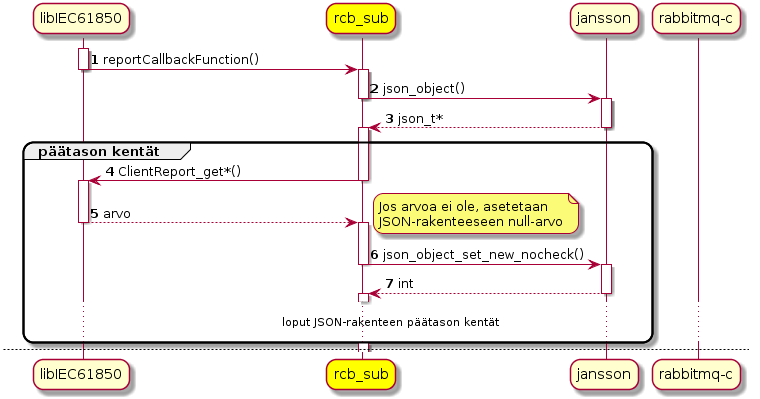
\includegraphics[width=1\textwidth]{pictures/rcb-sub-report-to-json.png}
	\caption{Sekvenssikaavio kuinka rcb\_sub muodostaa JSON:nin päätason kentät.}
	\label{fig:rcb-sub-report-to-json-1}
\end{figure}

Kuvassa \ref{fig:rcb-sub-report-to-json-1} suoritus alkaa kun libIEC61850-kirjasto kutsuu takaisinkutsufunktiota. Funktiolle annetaan parametrina saapunut viesti \emph{ClientReport}-struktuurin instanssina (kohta 1). Tämän jälkeen ohjelma käy läpi viestin jokaisen päätason kentän ja lisää ne JSON-rakenteeseen. Osa viestin kentistä on vaihtoehtoisia riippuen siitä, mitä käyttäjä asetti \texttt{-{}-opt\--\-fields} vivun parametrilla. Jos arvoa viestissä ei ole, korvataan se null-arvolla JSON:iin. Esimerkkinä liiteessä \ref{ch:report-json-format} rivillä 4 oleva \texttt{confRevision} muuttuja, jonka arvo on null. Tämän jälkeen suoritus jatkuu kuvasta \ref{fig:rcb-sub-report-to-json-1} kuvaan \ref{fig:rcb-sub-report-to-json-2}.

\begin{figure}[ht!]
	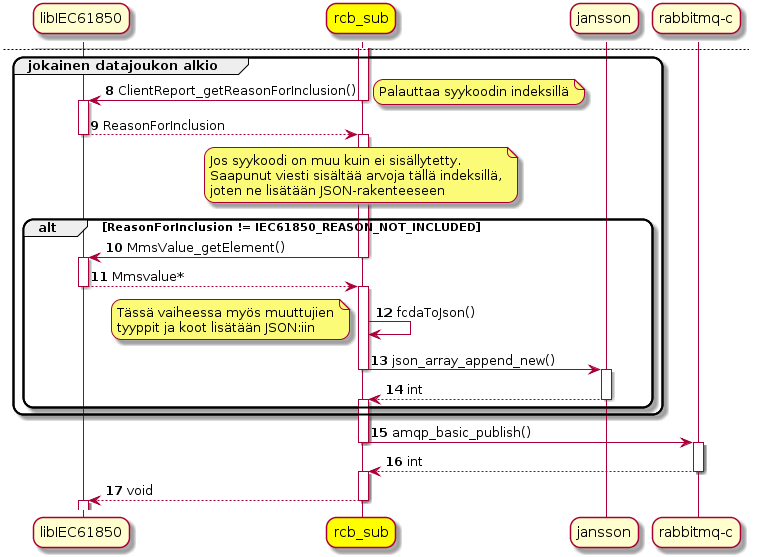
\includegraphics[width=1\textwidth]{pictures/rcb-sub-report-to-json_001.png}
	\caption{Sekvenssikaavio kuinka rcb\_sub lisää JSON:iin muuttujat viestistä.}
	\label{fig:rcb-sub-report-to-json-2}
\end{figure}

Päätason viestin kenttien jälkeen ohjelma käy läpi silmukassa viestin datajoukon indeksit (kuvassa \ref{fig:rcb-sub-report-to-json-2} kohdat 8--14). Viesti oikeasti sisältää vain ne datajoukon alkiot, jotka sisältyivät viestiin. Ongelmana tässä on se, että viesti ei sisällä indeksiä tai tietoa siitä mikä datajoukon alkio on kyseessä. Jotta tästä saadaan tieto, ohjelma pakottaa syykoodin päälle viestiin. Tämän avulla kun silmukassa käydään kaikki datajoukon indeksit läpi, voidaan jokaiselle indeksille ensin kysyä syykoodi viestistä (kohdat 8--9). Jos datajoukon alkio ei ole viestissä, palauttaa kirjaston funktio \texttt{Cli\-entRe\-port\-\_\-get\-Rea\-son\-For\-Inc\-lu\-si\-on\-()} arvon \texttt{IEC61850\_REASON\_NOT\_INCLUDED}. Tätä tietoa voidaan käyttää löytämään oikea datajoukon indeksi. Jos datajoukon indeksi on viestissä, suoritetaan kohdat 10--14, muuten mennään seuraavaan indeksiin ja toistetaan kohdat 8--9. Datajoukon indeksi tarvitaan, jotta aiemmin luetut spesifikaatiot saadaan yhdistettyä attribuutteihin arvojen kanssa. Datajoukon indeksillä, viestin arvoilla ja muuttujien tyypeillä ja koolla saadaan rakennettua loppuosa JSON-rakenteesta. Kuvassa \ref{fig:rcb-sub-report-to-json-2} oleva silmukka rakentaa liitteessä \ref{ch:report-json-format} olevan values-taulun alkaen riviltä 7. JSON:in sisempi values-taulu (rivi 13) on lista FCD- tai FCDA-viitteen muuttujia, mitä se viittaa arvoineen. Tämä taulukko muodostetaan kuvan \ref{fig:rcb-sub-report-to-json-2} kohdassa 12 funktiolla \texttt{fcdaToJson()} ja lisätään JSON:iin kohdassa 13. Lopuksi viesti lähetetään RabbitMQ-palvelimelle funktiolla \texttt{amqp\_basic\_publish()} ja takaisinkutsufunktio palaa (kohdat 15--17).

\section{Jatkokehitys}
Ohjelma jätettiin työssä pisteeseen, missä se saavutti kaikki sille asetetut vaatimukset. Kuitenkin tulevaisuudessa ohjelmaa voidaan lisätä ominaisuuksia tarpeen vaatiessa. Isoin puute ohjelmassa oli testiympäristö ja sen yksikkötestit. C:ssä ei ole suoraan tukea yksikkötestien kirjoittamiseen. Ympäristön pystytys vaatii erillisen kirjaston projektin yhteyteen, millä yksikkötestit kirjoitetaan. Tämä jäi tulevaisuuden kehitystyöksi ja ei sisältynyt tähän työhön. Yksikkötestit ovat kuitenkin tärkeä osa ohjelman ylläpitoa ja toiminnan varmistamista muutosten jälkeen. Testit tullaan tarvitsemaan ennemmin tai myöhemmin.

Ohjelma toteutettiin nyt niin, että se aina käyttää suoraa vaihdetyyppiä RabbitMQ-pal\-ve\-li\-mel\-la. Tämä täytti työlle asetetut vaatimukset. Jos tulevaisuudessa tarvitaan joustavuutta, voidaan ohjelmaan tehdä muutoksia ja parametreja lisätä helposti lisämään toiminnallisuutta. Esimerkkinä käyttäjä voisi valita käytettävän vaihteen tyypin parametrilla.